\documentclass[tikz,10pt]{standalone}
\usepackage{tkz-euclide}

\definecolor{ccred}{cmyk}{0, 0.87, 0.8, 0.21}
\definecolor{ccgreen}{RGB}{147,187,42}
\definecolor{ccgrey}{RGB}{158,155,155}

\begin{document}
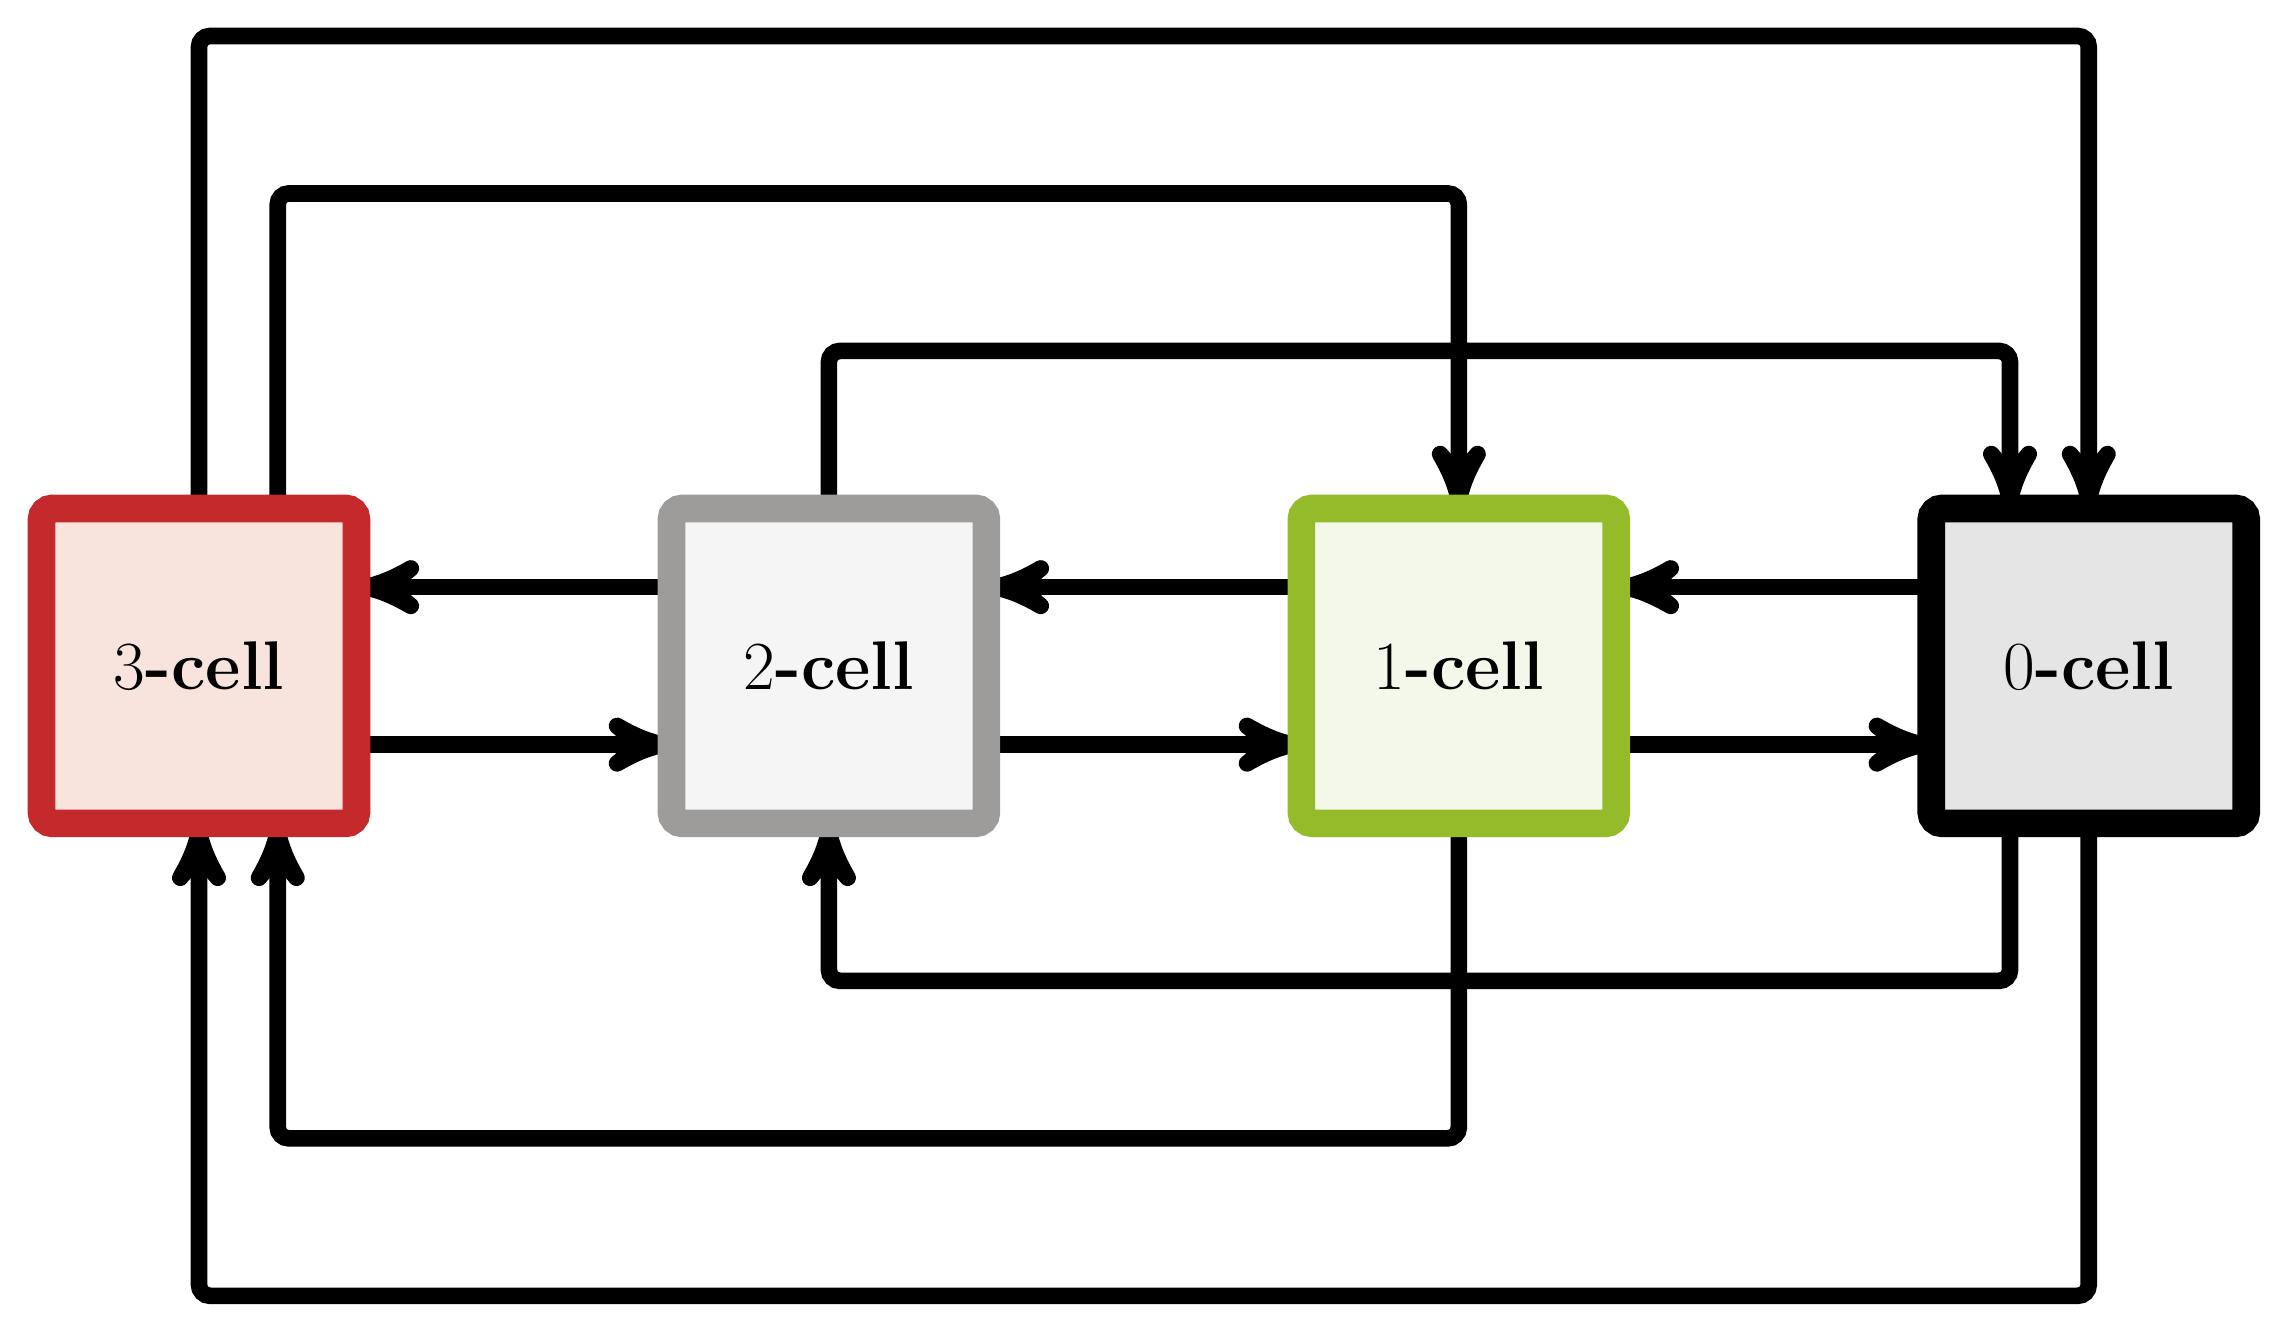
\begin{tikzpicture}[scale=2]

   % Style des flèches
  \tikzstyle{fleche} = [->, >=stealth', thick, rounded corners=4pt]
  \tikzstyle{doublefleche} = [<->, >=stealth', thick, rounded corners=4pt, line width=2]

    % R <-> F
  \draw[fleche, line width=6, black] (2,0.5) -- (4,0.5) ;
  \draw[fleche, line width=6, black] (4,1.5) -- (2,1.5) ;
  % F <-> E
  \draw[fleche, line width=6, black] (6,0.5) -- (8,0.5) ;
  \draw[fleche, line width=6, black] (8,1.5) -- (6,1.5) ;
  % E <-> N
  \draw[fleche, line width=6] (10,0.5) -- (12,0.5) ;
  \draw[fleche, line width=6] (12,1.5) -- (10,1.5) ;

  % N <-> F
  \draw[fleche, line width=6, black] (5,2) -- (5,3) -- (12.5,3) -- (12.5,2) ;
  \draw[fleche, line width=6, black] (12.5,0) -- (12.5,-1) -- (5,-1) -- (5,0) ;

  % E <-> R
  \draw[fleche, line width=6, black] (1.5,2) -- (1.5,4) -- (9,4) -- (9,2) ;
  \draw[fleche, line width=6, black] (9,0) -- (9,-2) -- (1.5,-2) -- (1.5,0) ;

  % N <-> R
  \draw[fleche, line width=6, black] (1,2) -- (1,5) -- (13,5) -- (13,2) ;
  \draw[fleche, line width=6, black] (13,0) -- (13,-3) -- (1,-3) -- (1,0) ;

  
  % Liste des boxes
  \draw[line width=10, ccred, rounded corners, fill=ccred!10!white] (0,0) -- (2,0) -- (2,2) -- (0,2) -- cycle ;
  \draw[line width=10, ccgrey, rounded corners, fill=ccgrey!10!white] (4,0) -- (6,0) -- (6,2) -- (4,2) -- cycle ;
  \draw[line width=10, ccgreen, rounded corners, fill=ccgreen!10!white] (8,0) -- (10,0) -- (10,2) -- (8,2) -- cycle ;
  \draw[line width=10, black, rounded corners, fill=black!10!white] (12,0) -- (14,0) -- (14,2) -- (12,2) -- cycle ;

  \draw (1,1) node (3cell) {\Huge \textbf{$3$-cell}};
  \draw (5,1) node (2cell) {\Huge \textbf{$2$-cell}};
  \draw (9,1) node (1cell) {\Huge \textbf{$1$-cell}};
  \draw (13,1) node (0cell) {\Huge \textbf{$0$-cell}};


\end{tikzpicture}
\end{document}